%!TeX root=../pridetop.tex
\chapter[Chapter \thechapter]{}
	
	
\begin{figure}[t!]
\centering

\includegraphics[width=.9\linewidth]{46top}
\captionlistentry{Headpiece to Chapter \thechapter}
\end{figure}


\lettrine[lines=6,image=true]{initials/chap46e}{lizabeth}  had been a good deal disappointed in not finding a letter from Jane on their first arrival at Lambton; and this disappointment had been renewed on each of the mornings that had now been spent there; but on the third her repining was over, and her sister justified, by the receipt of two letters from her at once, on one of which was marked that it had been mis-sent elsewhere. Elizabeth was not surprised at it, as Jane had written the direction remarkably ill.

They had just been preparing to walk as the letters came in; and her uncle and aunt, leaving her to enjoy them in quiet, set off by themselves. The one mis-sent must be first attended to; it had been written five days ago. The beginning contained an account of all their little parties and engagements, with such news as the country afforded; but the latter half, which was dated a day later, and written in evident agitation, gave more important intelligence. It was to this effect:—


\begin{quotation}
\indent Since writing the above, dearest Lizzy, something has occurred of a most unexpected and serious nature; but I am afraid of alarming you—be assured that we are all well. What I have to say relates to poor Lydia. An express came at twelve last night, just as we were all gone to bed, from Colonel Forster, to inform us that she was gone off to Scotland with one of his officers; to own the truth, with Wickham! Imagine our surprise. To Kitty, however, it does not seem so wholly unexpected. I am very, very sorry. So imprudent a match on both sides! But I am willing to hope the best, and that his character has been misunderstood. Thoughtless and indiscreet I can easily believe him, but this step (and let us rejoice over it) marks nothing bad at heart. His choice is disinterested at least, for he must know my father can give her nothing. Our poor mother is sadly grieved. My father bears it better. How thankful am I, that we never let them know what has been said against him; we must forget it ourselves. They were off Saturday night about twelve, as is conjectured, but were not missed till yesterday morning at eight. The express was sent off directly. My dear Lizzy, they must have passed within ten miles of us. Colonel Forster gives us reason to expect him here soon. Lydia left a few lines for his wife, informing her of their intention. I must conclude, for I cannot be long from my poor mother. I am afraid you will not be able to make it out, but I hardly know what I have written.
\end{quotation}


Without allowing herself time for consideration, and scarcely knowing what she felt, Elizabeth, on finishing this letter, instantly seized the other, and opening it with the utmost impatience, read as follows: it had been written a day later than the conclusion of the first.


\begin{quotation}
\indent By this time, my dearest sister, you have received my hurried letter; I wish this may be more intelligible, but though not confined for time, my head is so bewildered that I cannot answer for being coherent. Dearest Lizzy, I hardly know what I would write, but I have bad news for you, and it cannot be delayed. Imprudent as a marriage between Mr Wickham and our poor Lydia would be, we are now anxious to be assured it has taken place, for there is but too much reason to fear they are not gone to Scotland. Colonel Forster came yesterday, having left Brighton the day before, not many hours after the express. Though Lydia's short letter to Mrs F. gave them to understand that they were going to Gretna Green, something was dropped by Denny expressing his belief that W. never intended to go there, or to marry Lydia at all, which was repeated to Colonel F., who, instantly taking the alarm, set off from B., intending to trace their route. He did trace them easily to Clapham, but no farther; for on entering that place, they removed into a hackney-coach, and dismissed the chaise that brought them from Epsom. All that is known after this is, that they were seen to continue the London road. I know not what to think. After making every possible inquiry on that side London, Colonel F. came on into Hertfordshire, anxiously renewing them at all the turnpikes, and at the inns in Barnet and Hatfield, but without any success,—no such people had been seen to pass through. With the kindest concern he came on to Longbourn, and broke his apprehensions to us in a manner most creditable to his heart. I am sincerely grieved for him and Mrs F.; but no one can throw any blame on them. Our distress, my dear Lizzy, is very great. My father and mother believe the worst, but I cannot think so ill of him. Many circumstances might make it more eligible for them to be married privately in town than to pursue their first plan; and even if \textit{he} could form such a design against a young woman of Lydia's connections, which is not likely, can I suppose her so lost to everything? Impossible! I grieve to find, however, that Colonel F. is not disposed to depend upon their marriage: he shook his head when I expressed my hopes, and said he feared W. was not a man to be trusted. My poor mother is really ill, and keeps her room. Could she exert herself, it would be better, but this is not to be expected; and as to my father, I never in my life saw him so affected. Poor Kitty has anger for having concealed their attachment; but as it was a matter of confidence, one cannot wonder. I am truly glad, dearest Lizzy, that you have been spared something of these distressing scenes; but now, as the first shock is over, shall I own that I long for your return? I am not so selfish, however, as to press for it, if inconvenient. Adieu! I take up my pen again to do, what I have just told you I would not; but circumstances are such, that I cannot help earnestly begging you all to come here as soon as possible. I know my dear uncle and aunt so well, that I am not afraid of requesting it, though I have still something more to ask of the former. My father is going to London with Colonel Forster instantly, to try to discover her. What he means to do, I am sure I know not; but his excessive distress will not allow him to pursue any measure in the best and safest way, and Colonel Forster is obliged to be at Brighton again to-morrow evening. In such an exigence my uncle's advice and assistance would be everything in the world; he will immediately comprehend what I must feel, and I rely upon his goodness.
\end{quotation}


\begin{figure}[tbh]
\centering
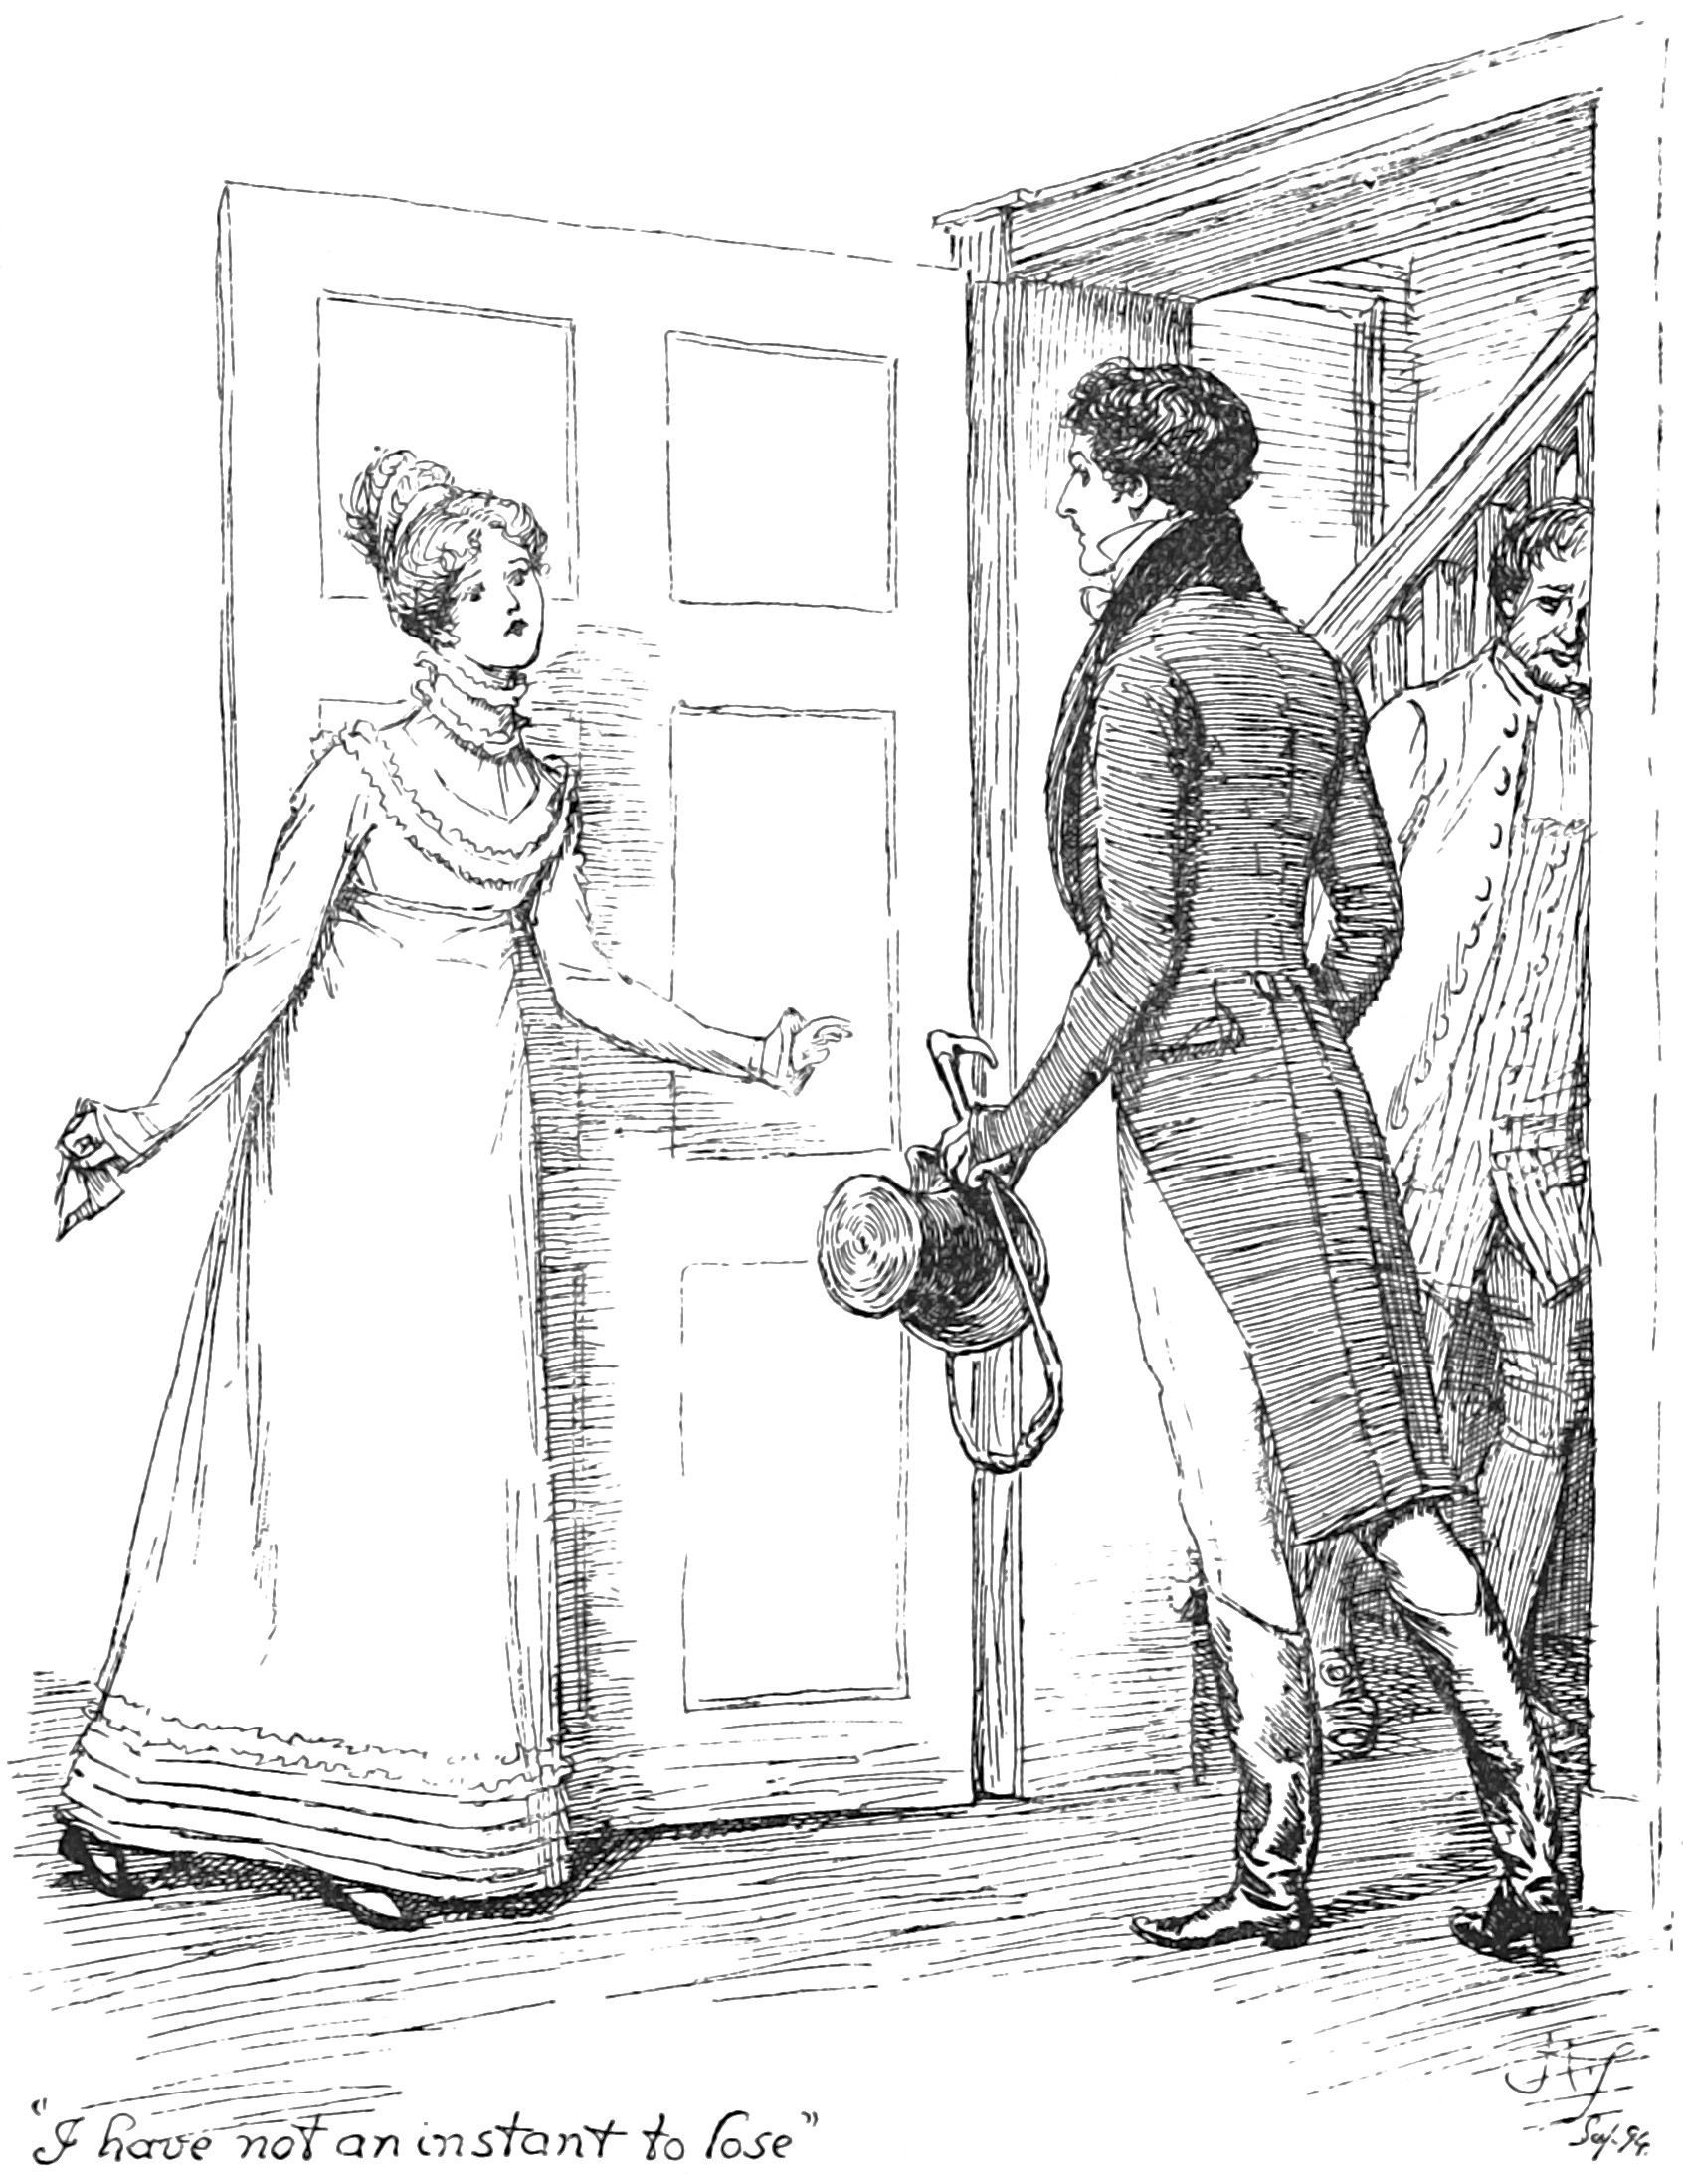
\includegraphics[width=.8\linewidth]{46instant}
\captionlistentry{»I have not an instant to lose«}
\end{figure}

»Oh! where, where is my uncle?« cried Elizabeth, darting from her seat as she finished the letter, in eagerness to follow him, without losing a moment of the time so precious; but as she reached the door, it was opened by a servant, and Mr Darcy appeared. Her pale face and impetuous manner made him start, and before he could recover himself enough to speak, she, in whose mind every idea was superseded by Lydia's situation, hastily exclaimed, »I beg your pardon, but I must leave you. I must find Mr Gardiner this moment on business that cannot be delayed; I have not an instant to lose.«

»Good God! what is the matter?« cried he, with more feeling than politeness; then recollecting himself, »I will not detain you a minute; but let me, or let the servant, go after Mr and Mrs Gardiner. You are not well enough; you cannot go yourself.«

Elizabeth hesitated; but her knees trembled under her, and she felt how little would be gained by her attempting to pursue them. Calling back the servant, therefore, she commissioned him, though in so breathless an accent as made her almost unintelligible, to fetch his master and mistress home instantly.

On his quitting the room, she sat down, unable to support herself, and looking so miserably ill, that it was impossible for Darcy to leave her, or to refrain from saying, in a tone of gentleness and commiseration, »Let me call your maid. Is there nothing you could take to give you present relief? A glass of wine; shall I get you one? You are very ill.«

»No, I thank you,« she replied, endeavouring to recover herself. »There is nothing the matter with me. I am quite well, I am only distressed by some dreadful news which I have just received from Longbourn.«

She burst into tears as she alluded to it, and for a few minutes could not speak another word. Darcy, in wretched suspense, could only say something indistinctly of his concern, and observe her in compassionate silence. At length she spoke again. »I have just had a letter from Jane, with such dreadful news. It cannot be concealed from anyone. My youngest sister has left all her friends—has eloped; has thrown herself into the power of—of Mr Wickham. They are gone off together from Brighton. \textit{You} know him too well to doubt the rest. She has no money, no connections, nothing that can tempt him to—she is lost for ever.«

Darcy was fixed in astonishment.

»When I consider,« she added, in a yet more agitated voice, »that \textit{I} might have prevented it! \textit{I} who knew what he was. Had I but explained some part of it only—some part of what I learnt, to my own family! Had his character been known, this could not have happened. But it is all, all too late now.«

»I am grieved, indeed,« cried Darcy: »grieved—shocked. But is it certain, absolutely certain?«

»Oh, yes! They left Brighton together on Sunday night, and were traced almost to London, but not beyond: they are certainly not gone to Scotland.«

»And what has been done, what has been attempted, to recover her?«

»My father has gone to London, and Jane has written to beg my uncle's immediate assistance, and we shall be off, I hope, in half an hour. But nothing can be done; I know very well that nothing can be done. How is such a man to be worked on? How are they even to be discovered? I have not the smallest hope. It is every way horrible!«

Darcy shook his head in silent acquiescence.

»When \textit{my} eyes were opened to his real character, oh! had I known what I ought, what I dared to do! But I knew not—I was afraid of doing too much. Wretched, wretched mistake!«

Darcy made no answer. He seemed scarcely to hear her, and was walking up and down the room in earnest meditation; his brow contracted, his air gloomy. Elizabeth soon observed, and instantly understood it. Her power was sinking; everything \textit{must} sink under such a proof of family weakness, such an assurance of the deepest disgrace. She could neither wonder nor condemn; but the belief of his self-conquest brought nothing consolatory to her bosom, afforded no palliation of her distress. It was, on the contrary, exactly calculated to make her understand her own wishes; and never had she so honestly felt that she could have loved him, as now, when all love must be vain.

But self, though it would intrude, could not engross her. Lydia—the humiliation, the misery she was bringing on them all—soon swallowed up every private care; and covering her face with her handkerchief, Elizabeth was soon lost to everything else; and, after a pause of several minutes, was only recalled to a sense of her situation by the voice of her companion, who, in a manner which, though it spoke compassion, spoke likewise restraint, said,—

»I am afraid you have been long desiring my absence, nor have I anything to plead in excuse of my stay, but real, though unavailing concern. Would to Heaven that anything could be either said or done on my part, that might offer consolation to such distress! But I will not torment you with vain wishes, which may seem purposely to ask for your thanks. This unfortunate affair will, I fear, prevent my sister's having the pleasure of seeing you at Pemberley to-day.«

»Oh, yes! Be so kind as to apologize for us to Miss Darcy. Say that urgent business calls us home immediately. Conceal the unhappy truth as long as it is possible. I know it cannot be long.«

He readily assured her of his secrecy, again expressed his sorrow for her distress, wished it a happier conclusion than there was at present reason to hope, and, leaving his compliments for her relations, with only one serious parting look, went away.

As he quitted the room, Elizabeth felt how improbable it was that they should ever see each other again on such terms of cordiality as had marked their several meetings in Derbyshire; and as she threw a retrospective glance over the whole of their acquaintance, so full of contradictions and varieties, sighed at the perverseness of those feelings which would now have promoted its continuance, and would formerly have rejoiced in its termination.

If gratitude and esteem are good foundations of affection, Elizabeth's change of sentiment will be neither improbable nor faulty. But if otherwise, if the regard springing from such sources is unreasonable or unnatural, in comparison of what is so often described as arising on a first interview with its object, and even before two words have been exchanged, nothing can be said in her defence, except that she had given somewhat of a trial to the latter method, in her partiality for Wickham, and that its ill success might, perhaps, authorize her to seek the other less interesting mode of attachment. Be that as it may, she saw him go with regret; and in this early example of what Lydia's infamy must produce, found additional anguish as she reflected on that wretched business. Never since reading Jane's second letter had she entertained a hope of Wickham's meaning to marry her. No one but Jane, she thought, could flatter herself with such an expectation. Surprise was the least of all her feelings on this development. While the contents of the first letter remained on her mind, she was all surprise, all astonishment, that Wickham should marry a girl whom it was impossible he could marry for money; and how Lydia could ever have attached him had appeared incomprehensible. But now it was all too natural. For such an attachment as this, she might have sufficient charms; and though she did not suppose Lydia to be deliberately engaging in an elopement, without the intention of marriage, she had no difficulty in believing that neither her virtue nor her understanding would preserve her from falling an easy prey.

She had never perceived, while the regiment was in Hertfordshire, that Lydia had any partiality for him; but she was convinced that Lydia had wanted only encouragement to attach herself to anybody. Sometimes one officer, sometimes another, had been her favourite, as their attentions raised them in her opinion. Her affections had been continually fluctuating, but never without an object. The mischief of neglect and mistaken indulgence towards such a girl—oh! how acutely did she now feel it!

She was wild to be at home—to hear, to see, to be upon the spot to share with Jane in the cares that must now fall wholly upon her, in a family so deranged; a father absent, a mother incapable of exertion, and requiring constant attendance; and though almost persuaded that nothing could be done for Lydia, her uncle's interference seemed of the utmost importance, and till he entered the room the misery of her impatience was severe. Mr and Mrs Gardiner had hurried back in alarm, supposing, by the servant's account, that their niece was taken suddenly ill; but satisfying them instantly on that head, she eagerly communicated the cause of their summons, reading the two letters aloud, and dwelling on the postscript of the last with trembling energy. Though Lydia had never been a favourite with them, Mr and Mrs Gardiner could not but be deeply affected. Not Lydia only, but all were concerned in it; and after the first exclamations of surprise and horror, Mr Gardiner readily promised every assistance in his power. Elizabeth, though expecting no less, thanked him with tears of gratitude; and all three being actuated by one spirit, everything relating to their journey was speedily settled. They were to be off as soon as possible. »But what is to be done about Pemberley?« cried Mrs Gardiner. »John told us Mr Darcy was here when you sent for us;—was it so?«

»Yes; and I told him we should not be able to keep our engagement. \textit{That} is all settled.«

»What is all settled?« repeated the other, as she ran into her room to prepare. »And are they upon such terms as for her to disclose the real truth? Oh, that I knew how it was!«

But wishes were vain; or, at best, could serve only to amuse her in the hurry and confusion of the following hour. Had Elizabeth been at leisure to be idle, she would have remained certain that all employment was impossible to one so wretched as herself; but she had her share of business as well as her aunt, and amongst the rest there were notes to be written to all their friends at Lambton, with false excuses for their sudden departure. An hour, however, saw the whole completed; and Mr Gardiner, meanwhile, having settled his account at the inn, nothing remained to be done but to go; and Elizabeth, after all the misery of the morning, found herself, in a shorter space of time than she could have supposed, seated in the carriage, and on the road to Longbourn.